\section{Structure of the equation}

This chapter follows 
\cite{convergence_of_allen_cahn_equation_to_multiphase_mean_curvature_flow}, 
but since the authors decided to only sketch some of the proofs, we will 
present more details.

Let $ \Lambda > 0 $ and define the flat torus 
$ \flattorus = [0, \Lambda )^{ d } = \mathbb{ R }^{ d } / \Lambda \mathbb{ Z 
}^{ d } $, 
which means that we work with periodic boundary conditions on $ \flattorus $.
Then for 
$ u \colon [ 0 , \infty ) \times \flattorus \to \mathbb{ R }^{ N } $ 
and some smooth potential 
$ W \colon \mathbb{ R }^{ N } \to [0, \infty ) $,
the \emph{Allen--Cahn equation} with parameter $ \varepsilon > 0 $ is given by
\begin{equation}
	\label{allen_cahn_eq}
	\partial_{ t } u 
	=
	\Delta u - \frac{1 }{ \varepsilon^{ 2 } } \nabla W ( u ).
\end{equation}
To understand this equation better, we consider the \emph{Cahn--Hilliard 
energy}, which assigns to $ u $ for a fixed time the value
\begin{equation}
	\label{cahn_hilliard_energy}
	\energy_{ \varepsilon } 
	(u)
	\coloneqq
	\int
	\frac{ 1 }{ \varepsilon }
	W ( u )
	+
	\frac{ \varepsilon }{ 2 }
	\abs{ \nabla u }^{ 2 }
	\dd{x}.
\end{equation}
Assume that everything is nice and smooth and that
$ u $ satisfies 
equation (\ref{allen_cahn_eq}). Then we have through an integration by parts 
that
\begin{align*}
	\dv{t} \energy_{ \varepsilon } ( u )
	&=
	\int
	\frac{ 1 }{ \varepsilon }
	\inner*{\nabla W ( u )}{ \partial_{ t } u}
	+
	\varepsilon
	\inner*{\nabla u}{ \nabla \partial_{ t } u}
	\dd{x}
	\\
	&=
	\int
	\inner*{ \frac{ 1 }{\varepsilon } \nabla W ( u ) - \varepsilon \Delta u  }{ \partial_{ t } u }
	\dd{x}
	\\
	&=
	\int - \varepsilon \abs{ \partial_{ t } u }^{ 2 } \dd{ x }
	\tag{\ref{allen_cahn_eq}}.
\end{align*}
For the last equality, we used that $ u $ solves the equation.
This calculation suggests that the partial differential equation 
(\ref{allen_cahn_eq}) is the $ \lp^{ 2 } $-gradient flow rescaled by $ 
\sqrt{\varepsilon} $ of the Cahn--Hilliard 
energy. Thus we can try to construct a solution to the PDE 
(\ref{allen_cahn_eq}) via De Giorgis minimizing movements scheme 
(\cite{de_giorgi_new_problems_on_minimizing_movements}), which we will do in 
\Cref{existence_of_ac_solution}.

But first we need to clarify what our potential $ W $ should look like. Classic 
examples in the scalar case are given by $ W ( u ) = \left( u^{ 2 } - 1 
\right)^{ 2 } $ or $ W( u ) = u^{ 2 } ( u - 1 )^{ 2 } $, and we call functions 
like these \emph{doublewell potentials}, see also 
\Cref{graph_of_doublewell_potential}.

\begin{figure}[ht]
	\centering
	\begin{tikzpicture}
		\begin{axis}[
			axis lines = left,
			xlabel = \(u\),
			ylabel = {\(W(u)= (u^2 - 1)^{ 2 }\)},
			]
			%Below the red parabola is defined
			\addplot [
			domain=-2:2, 
			samples=100, 
			color=black,
			]
			{x^4-2*x^2 + 1};
		\end{axis}
	\end{tikzpicture}
	\caption{Plot of the doublewell potential $ W(u) = (u^2 - 1 )^{ 2 } $}
	\label{graph_of_doublewell_potential}
\end{figure}

In higher dimensions, we want to accept the following potentials: $ W \colon 
\mathbb{ R }^{ N } \to [0, \infty ) $ has to be a smooth multiwell potential, 
meaning that it has finitely many zeros at $ u = \alpha_{ 1 }, \dotsc , 
\alpha_{ P } \in \mathbb{ R }^{ N } $. Furthermore we ask for polynomial growth 
in the sense that there exists some $ p \geq 2 $ such that for all $ u $ 
sufficiently large, we have
\begin{equation}
	\label{polynomial_growth}
	\abs{ u }^{ p } \lesssim W(u) \lesssim \abs{ u }^{ p }
\end{equation}
and
\begin{equation}
	\label{polynomial_growth_derivative}
	\abs{ \nabla W ( u ) } \lesssim \abs{ u }^{ p -1 }.
\end{equation}
Lastly we want $ W $ to be convex up to a small perturbation in the sense that 
there exist smooth functions 
$ W_{ \mathrm{conv} }$, $ W_{ \mathrm{pert} } \colon \mathbb{ R }^{ N } \to [ 0 , \infty ) $ such that
\begin{equation}
	\label{decomposition_of_w}
	W = W_{ \mathrm{conv}} + W_{ \mathrm{pert}}\, ,
\end{equation}
$ W_{ \mathrm{conv} } $ is convex and
\begin{equation}
	\label{perturbation bound}
	\sup_{ x \in \mathbb{ R }^{ N } }
	\abs{ \nabla^{ 2 } W_{ \mathrm{pert} } } < \infty.
\end{equation}
One can check that the above mentioned doublewell potentials satisfy these 
assumptions. In general one may consider potentials $ W $ of the form
\begin{equation*}
	W ( u ) \coloneqq
	\abs{ u - \alpha_{ 1 } }^{ 2 } 
	\cdot
	\dotsc
	\cdot
	\abs{ u - \alpha_{ P } }^{ 2 },
\end{equation*}
see also \Cref{twodimensional_potential} for the case $ P = 3 $ in two 
dimensions.
\begin{figure}[h]
	\centering
	
	\begin{subfigure}[b]{0.45\linewidth}
		
		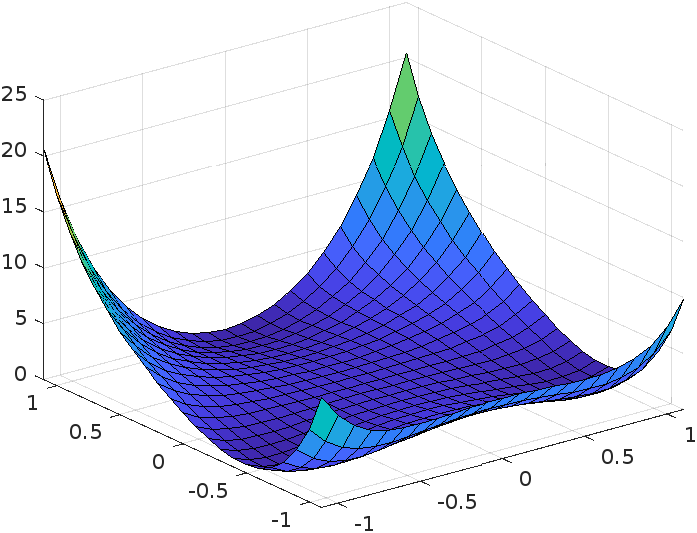
\includegraphics[width=\textwidth]{trianglepotentialsurf}
		\caption{Graph of the potential}
	\end{subfigure}
	\hfill
	\begin{subfigure}[b]{0.45\linewidth}
		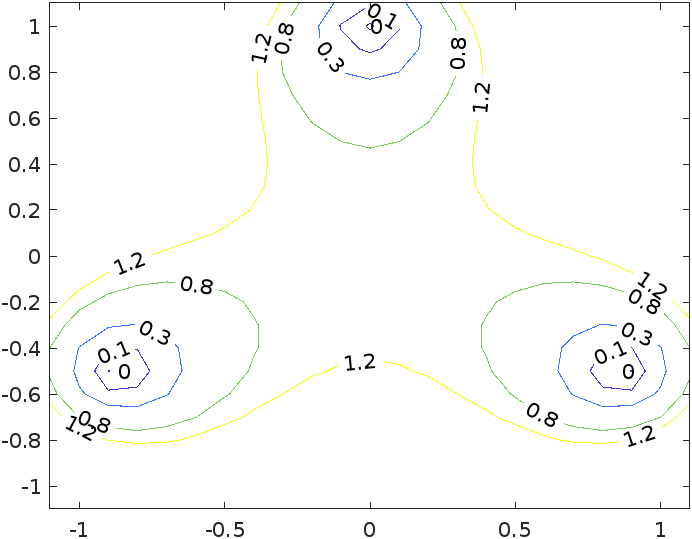
\includegraphics[width=\textwidth]{trianglecontour2d}
		
		\caption{Contour lines of the potential}
	\end{subfigure}
	
	\caption{Graphics for the potential
	$ W ( u ) = 
	\abs{ u  - e^{ i \pi\frac{ 3 }{ 6 }} }^{ 2 } 
	\abs{ u  - e^{ i \pi\frac{   7}{ 6  }} }^{ 2 }
	\abs{ u  - e^{ i \pi\frac{  11}{ 6  }} }^{ 2 }$ }
	\label{twodimensional_potential}
\end{figure} 
The existence of the function $ W_{ \mathrm{pert} } $ can then be seen by 
multiplying some suitable cutoff to $ W 
$ which is equal to 1 on a sufficiently large ball.

As it is custom for parabolic partial differential equations, we view solutions 
of the Allen--Cahn equation (\ref{allen_cahn_eq}) as maps from $ [0,T] $ into 
some suitable function space and thus use the following definition.

\begin{definition}
	\label{solution_to_ac}
	We say that a function 
	\begin{equation*}
	u_{ \varepsilon} \in 
	\mathrm{ C } \left( [0 , T ] ; \lp^{ 2 } \left( \flattorus; \mathbb{ R }^{ 
	N } \right) \right) \cap
	\lp^{ \infty } \left( [0, T ]; \wkp^{ 1, 2 } ( \flattorus ; \mathbb{ R }^{ 
	N } ) \right)
	\end{equation*}
	is a weak solution of the Allen--Cahn equation (\ref{allen_cahn_eq}) with parameter $ \varepsilon > 0 $ and initial condition $ u_{ \varepsilon}^{ 0 } \in \lp^{ 2 } ( \flattorus ; \mathbb{ R }^{ N } ) $ if
	\begin{enumerate}
		\item the energy stays bounded, which means that
		\begin{equation}
			\esssup_{ 0 \leq t \leq T }
			\energy_{ \varepsilon } ( u_{ \varepsilon } ( t ) ) 
			< \infty,
		\end{equation}
		\item 
		its weak time derivative satisfies
		\begin{equation}
			\partial_{ t } u_{ \varepsilon }
			\in
			\lp^{ 2 } \left( [ 0 , T ] \times \flattorus ; \mathbb{ R }^{ N } \right),
		\end{equation}
		\item 
		\label{here_appears_p}
		for almost every $ t \in [ 0 , T ] $ and every 
		$ \xi \in \lp^{ p } ( [ 0 , T ] \times \flattorus; \mathbb{ R }^{ N } ) 
		\cap
		\wkp^{ 1, 2 } ( [ 0, T ] \times \flattorus ; \mathbb{ R }^{ N } ) $,
		we have
		\begin{equation}
			\label{ac_weak_equation}
			\int
			\inner*{ \frac{ 1 }{ \varepsilon^{ 2 } } \nabla W ( u_{ \varepsilon} ( t ) ) }{ \xi }
			+
			\inner*{ \nabla u_{ \varepsilon } ( t ) }{ \nabla \xi } 
			+
			\inner*{\partial_{ t } u_{ \varepsilon} ( t ) }{ \xi }
			\dd{x}
			=
			0,
		\end{equation}
		\item 
		the initial conditions are attained in the sense that $ u_{ \varepsilon 
		} ( 0 ) = u_{ \varepsilon}^{ 0 } $.
	\end{enumerate}
\end{definition}

\begin{remark}
	The exponent $ p $ which appears in condition \ref{here_appears_p} is the 
	same 
	exponent as for the growth assumptions (\ref{polynomial_growth}) and 
	(\ref{polynomial_growth_derivative}) of $ W $.
	Moreover we note that given our setup, we automatically have $ \nabla W ( 
	u_{ \varepsilon } ) ( t ) \in \lp^{ p' } ( \flattorus ) $. In fact we can 
	estimate
	\begin{equation}
		\abs{ \nabla W ( u_{ \varepsilon} ) }^{ p/(p-1) }
		\lesssim
		1+ \abs{u_{ \varepsilon }}^{ p }
		\lesssim
		1 + W ( u ),
	\end{equation}
	which is integrable for almost every time $ t $ since we assume that the energy stays bounded,
	thus the integral in equation (\ref{ac_weak_equation}) is well defined.
	
	Moreover we already obtain $ 1/2 $ Hölder-continuity in time from the embedding
	\begin{equation}
		\label{w12_embeds_into_c1half}
		\wkp^{ 1 , 2} \left( [ 0 , T ] ; \lp^{ 2 } \left( \flattorus;\mathbb{ R 
		}^{ N } \right) \right)
		\hookrightarrow
		\cont^{ 1/2 } \left( [ 0 , T ] ; \lp^{ 2 } \left( \flattorus ; \mathbb{ 
		R 
		}^{ N } \right) \right),
	\end{equation}
	which follows from a generalized version of the fundamental theorem of calculus and Hölder's inequality.
\end{remark}